%%% PREAMBLE - Do not touch %%%%%%%%%%%%%%%%%%%%%%%%%%%%%%%%%%%%%%%%%%%%%%%%%%%%%%
\documentclass[10pt,twocolumn,letterpaper]{article}
\usepackage[utf8]{inputenc}
\usepackage[english]{babel}
\usepackage{model}
\usepackage{times}
\usepackage{epsfig}
\usepackage{graphicx}
\usepackage{amsmath}
\usepackage{textcomp}
\usepackage{amssymb}
\usepackage{color}
\usepackage[pagebackref=true,breaklinks=true,letterpaper=true,colorlinks,bookmarks=false]{hyperref}

%% inset source code
\usepackage{listings}

\lstset{basicstyle=\footnotesize\ttfamily,  language=C}
\renewcommand{\lstlistingname}{Code}% Listing -> Algorithm

\let\url\nolinkurl% Make \url be equivalent to \nolinkurl
\newcommand*{\Package}[1]{\texttt{#1}}%

\cvprfinalcopy % *** Uncomment this line for the final submission
\def\httilde{\mbox{\tt\raisebox{-.5ex}{\symbol{126}}}}
\ifcvprfinal\pagestyle{empty}\fi

\newcommand{\TODO}[1]{TODO: #1}
\newcommand{\CITEONE}[2]{\mbox{#1 \cite{#2}}}
\newcommand{\CITETWO}[3]{\mbox{#1 and #2 \cite{#3}}}
\newcommand{\CITEN}[2]{\mbox{#1 et al. \cite{#2}}}

%%% Report beginning %%%%%%%%%%%%%%%%%%%%%%%%%%%%%%%%%%%%%%%%%%%%%%%%%%%%%%%%%%%%%%
\begin{document}

%%% Title and authors %%%%%%%%%%%%%%%%%%%%%%%%%%%%%%%%%%%%%%%%%%%%%%%%%%%%%%%%%%%%
\title{Relatório do projeto 2: Gerenciamento e Cruzamento}
\author{Isadora Sophia Garcia Rodopoulos \thanks{RA 158018, Instituto de Computação, Universidade de Campinas, Unicamp. \textbf{Contact}: \tt\small{isadorasophiagr@gmail.com}} \\
Matheus Mortatti Diamantinos \thanks{RA 156740, Instituto de Computação, Universidade de Campinas, Unicamp. \textbf{Contact}: \tt\small{matdiamantino@gmail.com}}\\
Luiz Fernando Bittencourt\thanks{MC833, Instituto de Computação, Universidade de Campinas, Unicamp. \textbf{Contact}: \tt\small{bit@ic.unicamp.br }}\\
}

%%% Abstrato %%%%%%%%%%%%%%%%%%%%%%%%%%%%%%%%%%%%%%%%%%%%%%%%%%%%%%%%%%%%%%%%%%%%%
\maketitle
\begin{abstract}
O objetivo do trabalho foi a implementação de um gerenciamento de trânsito e cruzamento, analisando o \textit{trade-off} e a performance do algoritmo desenvolvido, além de seu impacto no mundo real.
\end{abstract}

%%% image for demo! %%%%%%%%%% 
\begin{figure*}
\begin{center}
    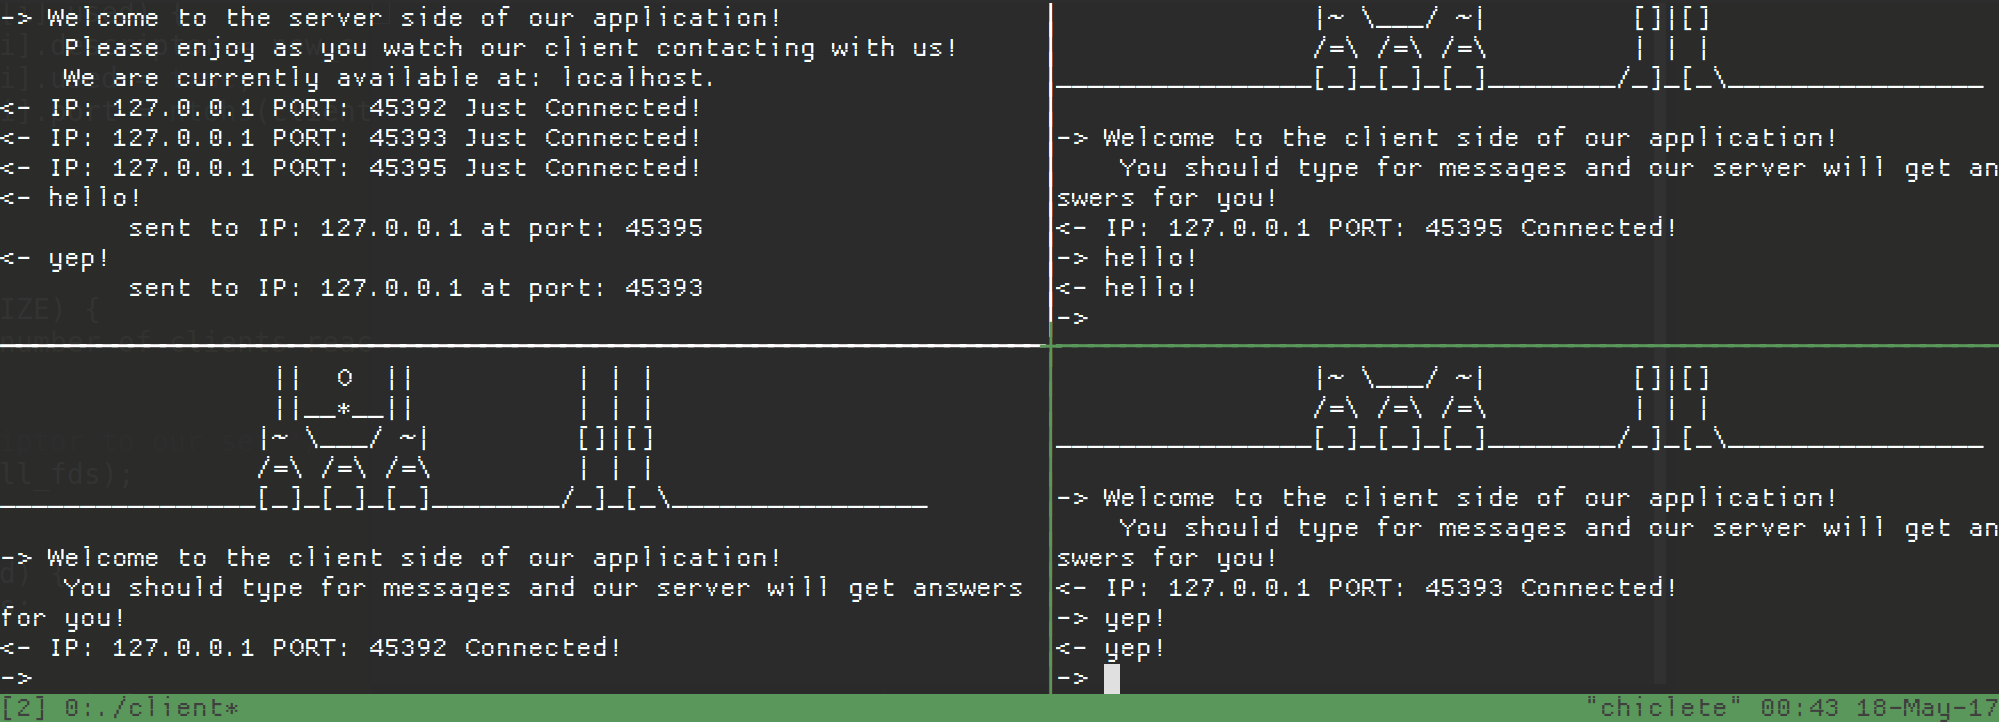
\includegraphics[width=1\textwidth]{img/sample.png}
    \caption{Exemplo de funcionamento do projeto}   
\end{center} 
\end{figure*}
%%%%%%%%%%%%%%%%%%%%%%%%%%%%%%%%%% page 2

%%% Introdução %%%%%%%%%%%%%%%%%%%%%%%%%%%%%%%%%%%%%%%%%%%%%%%%%%%%%%%%%%%%%%%%%%%
Neste projeto, foi implementado um sistema cliente-servidor onde cada cliente representa um carro atravessando um cruzamento de mão dupla e o servidor fica responsável por processar três tipos de requisitos dos carros: \textbf{segurança}, \textbf{entretenimento} e \textbf{tráfego}.

Os pacotes de segurança são os responsáveis por pedir informações de trânsito, mandando a posição e velocidade do carro. O servidor, ao receber este pacote, calcula se uma colisão ocorrerá ou se já ocorreu, mandando um comando ao carro que fez a requisição com uma das seguintes ações: 

\begin{itemize}
    \item acelerar; 
    \item freiar;
    \item chamar Ambulância.
\end{itemize}

%%% Seções %%%%%%%#####%%%%%%%%%%%%%%%%%%%%%%%%%%%%%%%%%%%%%%%%%%%%%%%%%%%%%%%%%%%
\section{Métodos}
Os métodos utilizados neste projeto podem ser separados em duas categorias: \textbf{comunicação} e \textbf{detecção de colisão}. A seguir, cada categoria é detalhada.

\subsection{Comunicação}
    O estabelecimento da comunicação entre cliente e servidor é feita utilizando o protocolo TCP, de modo que os pacotes cheguem garantidamente nas duas pontas da comunicação. Contudo, a troca de mensagens pode ter uma duração maior, fazendo com que os comandos de trânsito demorem mais para serem executados.

    \subsubsection{Cliente}
        O cliente realiza requisições ao servidor de dois tipos: Segurança e Outros, onde Segurança diz respeito a pacotes que pedem informações de trânsito e Outros são os pacotes de conforto e tráfego, com prioridade mais baixa. As prioridades são definidas de acordo com a latência de processamento e comunicação, sendo definidas como > 100ms para as prioridades mais baixas e < 10ms para as prioridades mais altas. Deste modo, é possível receber informações de trânsito com mais frequência e com menos atraso, obtendo uma confiabilidade maior nos carros autônomos.
        
        Para simular tal prioridade, foi definida uma variável de tempo que nos diz o quanto tempo é necessário esperar antes de mandar outro pacote, dependendo do tipo deste:

\begin{lstlisting}[caption={Demonstração do código para o envio de pacotes}, label=Algorithm]
if (time_passed(last_sent_security, 
        my_car.cur_time) >= latency(SECURITY)) {
    /* send security packet */
}

if (time_passed(last_sent_other, 
        my_car.cur_time) >= latency(OTHER)) {
    /* send any other packet */
}
\end{lstlisting}

    \subsubsection{Servidor}
        O servidor utiliza a estrutura \texttt{select} implementada na atividade \textbf{2.2} para se comunicar com diversos clientes ao mesmo tempo, de modo a calcular possíveis colisões para cada um dos clientes que estão trafegando pelo cruzamento. A estrutura funciona olhando para cada socket de comunicação de cada cliente ativo e verificando se alguma mensagem chega de algum deles. Se sim, verifica o tipo da mensagem. Se a mensagem for do tipo \textit{segurança}, verifica colisão para algum dos clientes ativos e manda os comandos necessários aos carros que estão sujeitos a colisão. Se for do tipo \textit{outros}, simula o processamento desta requisição processando uma função que roda por um tempo fixo sem realizar nenhuma atividade significativa, e então retorna um pacote sem informações úteis.
            
\subsection{Detecção de colisão}
    Para realizar a detecção de colisão, primeiro discutimos a estrutura de dados utilizada para definir um carro.

\begin{lstlisting}[caption={Estrutura utilizada para a descrição de um carro}, label=Algorithm]
typedef enum { LOW=9, HIGH=100 } Latency;
typedef enum { SECURITY=1, ENTERTAINMENT=2, 
               COMFORT=3, OTHER=4 } Type;

typedef struct {
    struct timespec cur_time;
    int64_t break_time;
    int32_t command, size; 
    int32_t x, y, 
            vx, vy, 
            dirx, diry;

    Type type;
} Car;
\end{lstlisting}

    Nesta estrutura, temos o timestamp do carro (\texttt{cur\_time}), o tempo em que o carro precisa ficar parado em caso de comando de freio (\texttt{break\_time}), o comando que ele deve realizar (\texttt{command}) e variáveis que representam a posição (\texttt{x}, \texttt{y}), direção e velocidade (unidades por segundo) do carro.

    Cada carro atualiza sua própria posição toda vez que o contador do respectivo cliente passa de 1 segundo. Então, a função \texttt{update\_car()} é chamada.

\begin{lstlisting}[caption={Código para a atualização de um carro}, label=Algorithm]
/* * update car for /n/ iterations */
void update_car_n(Car *car, int n) {
    car->x += n*car->vx;
    car->y += n*car->vy;
}
\end{lstlisting}

    Cada cliente recebe um arquivo de entrada com as seguintes informações:

    \begin{enumerate}
        \item quantidade de updates para as informações do carro;
        \item tamanho do carro;
        \item posição x;
        \item posição y;
        \item velocidade x;
        \item velocidade y;
        \item tempo de duração total
    \end{enumerate}

    E a cada intervalo de tempo definido nesta entrada, lê a próxima velocidade definida. Após os inputs terminarem, se necessário, uma velocidade padrão é definida para o carro.

    No lado do servidor, então, ao receber um novo pacote de segurança do cliente, possíveis colisões com os diversos carros da pista são verificados a partir dos métodos a seguir.

    Inicialmente, são atualizadas as posições dos carros que estão conectados a partir do timestamp da última mensagem recebida.

\begin{lstlisting}[caption={Código para atualização dos carros}, label=Algorithm]
/* update cars */
for (i = 0; i < size; i++) {
    int64_t elapsed = since_now(cars[i].cur_time);
    clock_gettime(CLOCK_REALTIME, &cars[i].cur_time);
    update_car_n(&cars[i], elapsed);
}
\end{lstlisting}

    Isto garantirá que o servidor saiba onde os outros carros estão mesmo se estes não mandaram mensagens a ele. Contudo, os carros podem ter mudado a velocidade sem o servidor saber e, portanto, isto é apenas uma previsão de onde os carros podem estar no tempo atual.
    
    Então,  é verificado para cada dupla de carros se os carros i e j já se colidiram ou se estão a colidir.

\subsection{Colisão}
    Para detectar se a colisão ocorreu, observe a figura abaixo:

\begin{figure}[ht!]
    \center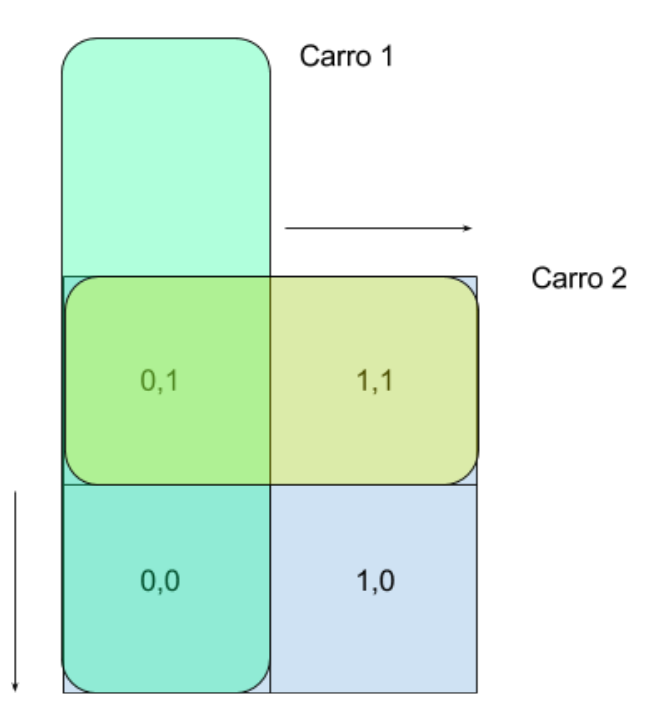
\includegraphics[width=.5\hsize]{img/car-vis}
    \caption{Modelo de visualização dos veículos}
\end{figure}

    Podemos ver na figura que podemos verificar a colisão no ponto (0, 1) verificando se este ponto está dentro do intervalo de tamanho dos dois carros ao mesmo tempo. Para isso, podemos observar que o intervalo [(x1, y1), (x2, y2)] que representam os pontos da frente e da traseira do carro precisam conter o ponto (0, 1), conforme a imagem. Logo, generalizando, foi implementado a verificação abaixo:

\begin{lstlisting}[caption={Algoritmo de detecção de colisão (1)}, label=Algorithm]
/* check if already collided! */
if (source.vy > 0)
    cond_s = source.y >= y 
        && source.y <= y + source.size;
else
    cond_s = source.y <= y 
        && source.y >= y - source.size;

if (target.vx > 0)
    cond_t = target.x >= x 
        && target.x <= x + target.size;
else
    cond_t = target.x <= x 
        && target.x >= x - target.size;

if (cond_s && cond_t) {
    *car1 = i;
    *car2 = j;
    return AMBULANCE;
}
\end{lstlisting}

    Observe que, dependendo da direção do carro, temos uma verificação diferente. Por exemplo, para o carro que está andando no eixo y com velocidade positiva, verificamos se a frente do carro já passou do ponto P e se a traseira ainda não passou. Assim, sabemos que o carro ainda está passando no cruzamento e podemos detectar se houve uma colisão entre dois carros. Se houver, mandamos o comando para chamar a ambulância aos dois carros que estão envolvidos no acidente.
    
    Então, se não houve acidente, precisamos verificar se um acidente irá ocorrer, baseado no tempo que cada carro vai demorar para entrar e sair do cruzamento.

\begin{figure}[ht!]
    \center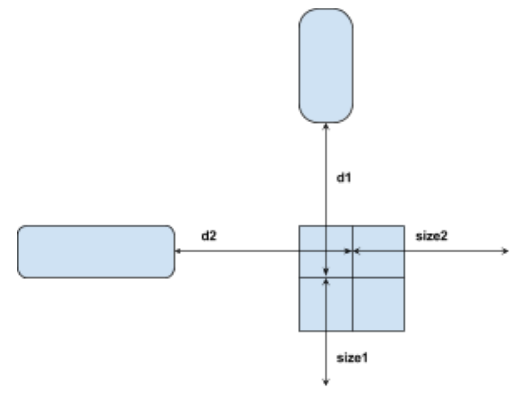
\includegraphics[width=.5\hsize]{img/car-cal}
    \caption{Modelo de cálculo de colisão dos veículos}
\end{figure}

    Conforme a imagem acima, precisamos saber o tempo que demora para o carro 1 andar a distância d1  e o tempo que demora para ele andar a distância d1 + size1 (tamanho do carro). Deste modo, podemos verificar se os intervalos de tempo para o carro 1 e o 2 entrar e sair do cruzamento de intersectam e, então se os carros irão se colidir quando entrarem no cruzamento.

\begin{lstlisting}[caption={Continuação do algoritmo de detecção de colisão (2)}, label=Algorithm]
/* source */
int dy = y - source.y;
int64_t time_in_s = 
    DIVZERO(dy, source.vy);

dy = (y + sign(source.vy)*source.size) 
        - source.y;
int64_t time_out_s =
    DIVZERO(dy, source.vy);

/* target */
int dx = x - target.x;
int64_t time_in_t = 
    DIVZERO(dx, target.vx);

dx = (x + sign(target.vx)*target.size) 
        - target.x;
int64_t time_out_t = 
    DIVZERO(dx, target.vx);
\end{lstlisting}

Foi implementado o cálculo do tempo utilizando a equação:

\begin{equation}
\cfrac{\Delta S}{V} = \Delta T
\end{equation}

    ...que nos retorna o tempo necessário para andar dS unidades andando com velocidade V.
    
    Então, se os intervalos se intersectam, mandamos para um dos carros o comando de freio junto com um intervalo de tempo no qual ele deve ficar parado. Este intervalo é calculado verificando o imaior intervalo de tempo entre o carro 1 e o 2 entrarem e sairem do cruzamento.

\begin{lstlisting}[caption={Continuação do algoritmo de detecção de colisão (3)}, label=Algorithm]
if (time_in_s <= time_out_t 
        && time_in_t <= time_out_s) {
    *car1 = i;
    cars[i].break_time = 
        1000* max(abs(time_in_t - time_out_t), 
                  abs(time_in_s - time_out_s));
    
    return BREAK;
 }
\end{lstlisting}

Caso não são detectadas colisões, apenas pede ao carro que chama a função continuar acelerando.

%%% Results&etc %%%%%%%%%%%%%%%%%%%%%%%%%%%%%%%%%%%%%%%%%%%%%%%%%%%%%%%%%%%%%%%%%
%%
\section{Resultados e discussão}
Para a validação da corretude do programa, foram executados diversos testes de fim a determinar a efetividade do nosso sistema de trânsito desenvolvido.

%%% References %%%%%%%%%%%%%%%%%%%%%%%%%%%%%%%%%%%%%%%%%%%%%%%%%%%%%%%%%%%%%%%%%
%%
{\small
\bibliographystyle{unsrt}
\bibliography{refs}
}

\end{document}
